\chapter{Sliced Mixed-Marginal Wasserstein}


\section{Abstract}
	Multi-marginal optimal transport enables one to compare multiple probability measures, which increasingly finds application in multi-task learning problems.
	One practical limitation of multi-marginal transport is computational scalability in the number of measures, samples and dimensionality.
	In this work, we propose a multi-marginal optimal transport paradigm based on random one-dimensional projections, whose (generalized) distance we term the \emph{sliced multi-marginal Wasserstein distance}.
	To construct this distance, we introduce a characterization of the one-dimensional multi-marginal Kantorovich problem and use it to highlight a number of properties of the sliced multi-marginal Wasserstein distance. 
	In particular, we show that (i) the sliced multi-marginal Wasserstein distance is a (generalized) metric that induces the same topology as the standard Wasserstein distance, (ii) it admits a dimension-free sample complexity, (iii) it is tightly connected with the problem of barycentric averaging under the sliced-Wasserstein metric.
	We conclude by illustrating the sliced multi-marginal Wasserstein on multi-task density estimation and multi-dynamics reinforcement learning problems.

\section{Introduction}

Optimal transport is a framework for defining meaningful metrics between probability measures \cite{villani, compopt}. 
These metrics find a wide range of applications, such as generative modeling \cite{pmlr-v84-genevay18a,bunne2019}, Bayesian inference \cite{bayes}, imitation learning \cite{Dadashi2020PrimalWI}, graph matching and averaging \cite{pmlr-v97-xu19b,NIPS2019_8569}.
Multi-marginal optimal transport \cite{gangbo} studies ways of comparing more than two probability measures in a geometrically meaningful way.
Multi-marginal distances defined using this paradigm are often useful in settings where sharing geometric structure is useful, such as multi-task learning. In particular, they have been applied for training multi-modal generative adversarial networks \cite{mwgan}, clustering  \cite{generalizedmet}, and computing barycenters of measures \cite{altschuler_mm}.


Following the establishment of key theoretical results, including by \textcite{gangbo,journals/siamma/AguehC11, Pass2014MultimarginalOT}, research is shifting toward applications. This motivates a need for practical algorithms for the multi-marginal setting \cite{mw_compl}. 
Standard approaches based on linear programming and entropic regularization scale exponentially with the number of measures, and/or the dimension of the space \cite{benamou:hal-01096124, accmmot}. 
A number of recent works have therefore studied settings, where multi-marginal transport problems can be efficiently solved via low-rank structures on the underlying cost function \cite{altschuler_mm}, but exponential cost in the dimension remains \cite{altschulernpbary, altschuler_mm_np}. 


In parallel, a number of works on \emph{sliced transport} \cite{bonnottee} developed techniques for scalable transport, which (i) derive a closed form for a problem in a single dimension, and (ii) extend it into higher dimensions via random linear projections (slicing) and thereby inherit the complexity of the one-dimensional problem.
This strategy has been shown effective in the classical Wasserstein \cite{bonnottee,bonneel, gensliced, distributionalsliced, maxsliced, orthsliced} and Gromov--Wasserstein \cite{sliced_gw} settings between pairs of measures, but has not yet been applied to settings with more than two measures.


In this paper, we address this gap and propose \emph{sliced multi-marginal transport}, providing a scalable analog of the multi-marginal Wasserstein distance.
To do so, we derive a closed-form expression for multi-marginal Wasserstein transport in one dimension, which lifts to a higher-dimensional analog via slicing. 
This one-dimensional closed-form expression can be computed with a complexity of $\mathcal{O}(PN\log N)$, where $P$ is the number of measures and $N$ is the number of samples per measure. 
Sliced multi-marginal Wasserstein ($\mathcal{SMW}$) can be estimated by Monte Carlo in $\mathcal{O}(KPN\log N)$, where $K$ is the number of Monte Carlo samples. 

Furthermore, we study $\mathcal{SMW}$'s theoretical properties.
We prove that (i) it is a generalized metric, whose associated topology is the topology of weak convergence, (ii) its sample complexity is dimension free, just like the sliced Wasserstein case involving two measures, and (iii) sliced multi-marginal transport is closely connected with the problem of barycentric averaging under the sliced Wasserstein metric. 
% Furthermore, we discuss projection complexity, and inequalities that relate sliced multi-marginal optimal transport with the Wasserstein distance between the marginals. 
%
We also showcase applications, where we focus on multi-task learning on probability spaces, where sharing knowledge across tasks can be beneficial and sliced multi-marginal Wasserstein can be used as a regularizer between task-specific models. 
We demonstrate this on a multi-task density estimation problem, where individual estimation tasks are corrupted and shared structure is needed to solve the problem, as well as a reinforcement learning problem, where certain agents receive no reward and must instead learn from other agents to solve their given task.


\section{Background}

\label{sec:background}

Multi-marginal optimal transport \cite{gangbo} is a class of optimization problems for comparing multiple measures $\mu_1,\ldots,\mu_P \in \mathcal{M}(\R^d)$, all supported on the metric space $(\R^d,  || \cdot||_2)$. 
The most common such problem is computing the multi-marginal Wasserstein distance, defined as
\[
\label{eq:multi_marginal_w}
\mathcal{MW}^2(\mu_1,\ldots,\mu_P)=\min_{\pi \in \Pi(\mu_1,\ldots, \mu_P)} \int_{(\mathbb{R}^d)^P}  c(x_1,\ldots,x_P) \, d\pi(x_1,\ldots,x_P),
\]

where $c:\mathbb{R}^d \times\ldots\times \mathbb{R}^d \to \mathbb{R}$ is a cost function and $\Pi(\mu_1,\ldots, \mu_P)$ is the set of probability measures in $\mathcal{M}((\mathbb{R}^d)^P)$ with marginals $\mu_1, \ldots, \mu_P$.
We focus on the barycentric cost of \textcite{gangbo, journals/siamma/AguehC11}, given by
\[
c(x_1,\ldots,x_P) = \sum_{p=1}^P \beta_p \Big\Vert  x_p - \sum_{j=1}^P\beta_j x_j\Big\Vert ^2,
\quad\beta_1,\ldots,\beta_P \geq 0, \quad \sum_{p=1}^P \beta_p = 1
.
\]
This cost was originally motivated from an economics-inspired perspective, but is also often preferable because it leads to connections with barycentric averaging \cite{journals/siamma/AguehC11}, giving it a simple interpretation.
It also recovers the Wasserstein distance with squared $2$-Euclidean cost in the case $P=2$ (up to constants), referred to as $\mathcal{W}$.
Algorithms for estimating \eqref{eq:multi_marginal_w} from a set of samples  scale exponentially with the number of measures $P$ and/or the dimension $d$ of the ground space  \cite{altschuler_mm, altschulernpbary, benamou:hal-01096124}.

$\mathcal{MW}$ is useful in multi-task settings for regularizing measures $\mu_1,\ldots, \mu_P$ by adding $\mathcal{MW}(\mu_1,\ldots, \mu_P)$ to a multi-task loss. 
It can also be used in a setting, where we aim for a model output $\mu$ to be close to a given set of measures $\nu_1,\ldots, \nu_P$, which can be done by introducing a loss of the form $\mathcal{MW}(\mu, \nu_1,\ldots, \nu_P)$ and minimizing it with respect to $\mu$.


% \begin{center}
% \begin{tabular}{llll}
% Method (incl. reference) & Computational complexity & Comments\\
% \end{tabular}
% \end{center}

\begin{figure}
	\centering
	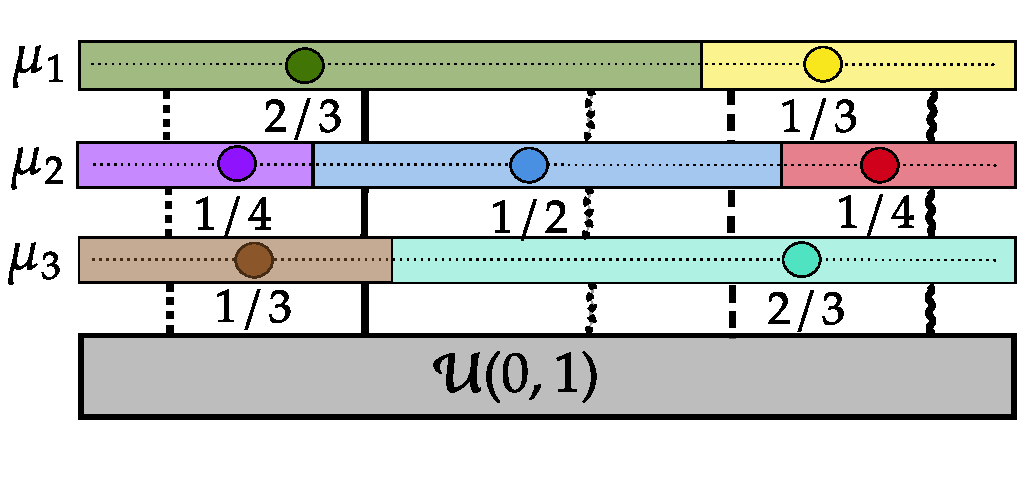
\includegraphics[height=3cm]{pictures/diagrams/diagram_uniform.pdf}
	\hspace{5mm}
	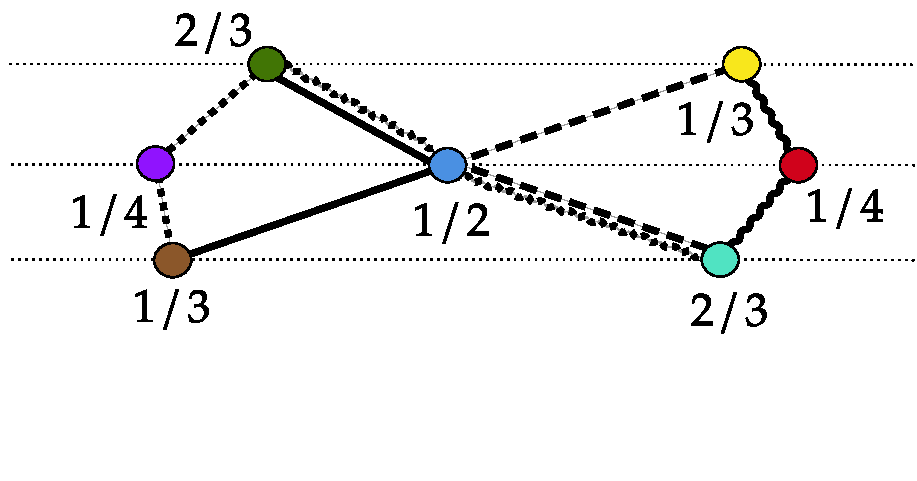
\includegraphics[height=3cm]{pictures/diagrams/diagram_alignment.pdf}
	% 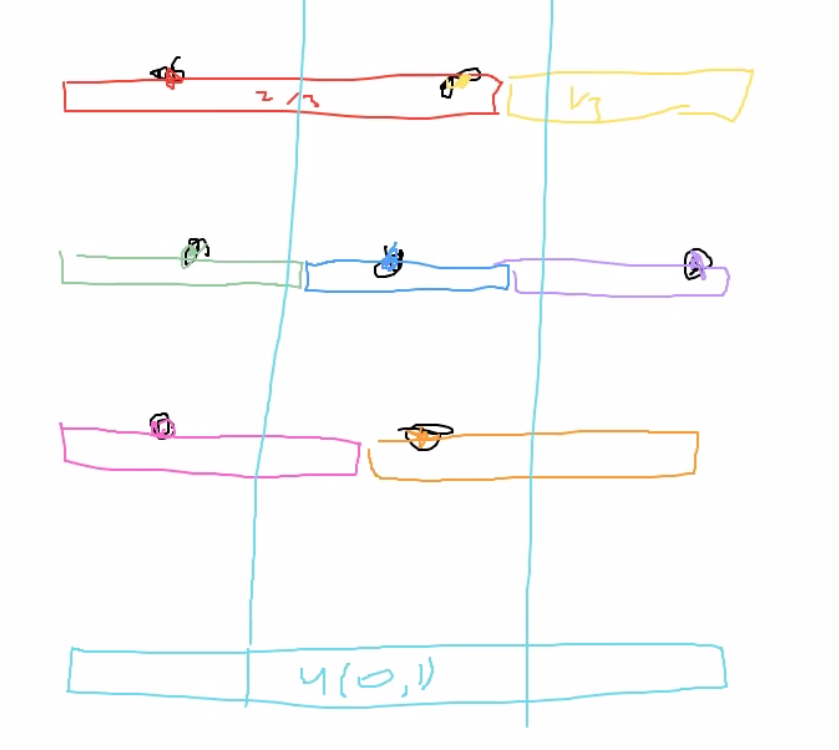
\includegraphics[width=\hsize]{images/diagrams/sketch}
	\caption{Illustration of the optimal coupling's structure on $\R$ between discrete measures $\mu_1, \mu_2$ and $\mu_3$. Points are samples of each measures, with weights next to them.  Left: histogram of measures (horizontal); joint samples are obtained by sampling a (black) line uniformly (drawn vertically), and picking points that are associated with the bin intersected by that line. Right: Corresponding triples of points that are aligned according to the coupling are linked by a pair of lines.}
	\label{fig:illustr_mmot}
\end{figure}
%\subsection{Slicing Techniques for Scalability}
\textbf{Sliced transport.}  With the usual Euclidean-type cost structures, the Wasserstein distance between pairs of one-dimensional discrete measures can be computed efficiently using \emph{sorting}  with $\mathcal{O}(N \log N)$ complexity.
More generally, we can consider the average distance between measures projected onto $\mathbb{R}$ along random axis, which gives \cite{bonnottee, bonneel}
\[
\mathcal{SW}^2(\mu, \nu) = \int_{S_{d-1}}\mathcal{W}^2\big(M^{\theta}_{\#}(\mu), M^{\theta}_{\#}(\nu)\big) \, d\Theta(\theta),
\]
where $M^{\theta}(x) = x^T \theta$, $(.)_\#$ denotes the push-forward of measures, and $\Theta$ is the uniform distribution on the unit sphere $S_{d-1}$. We sample from $M^{\theta}_{\#}(\mu)$ by sampling from $\mu$ and  projecting onto $\theta$.


A fundamental result by \textcite{bonnottee} is that $\mathcal{SW}$ is a metric that metrizes the topology of weak convergence---the \emph{exact same} topology as $\mathcal{W}$.
$\mathcal{SW}$ can be estimated via Monte Carlo and preserves the computational complexity of estimating $\mathcal{W}$ on $\R$, which is $\mathcal{O}(N\log N)$.
Owing to the Monte Carlo nature, the sample complexity of $\mathcal{SW}$ is dimension free \cite{bonnottee, topstatprop}, in contrast with the exponential dependency of the Wasserstein distance on dimension.
The combination of good computational and statistical properties makes $\mathcal{SW}$ an attractive choice for  minimization problems on measure spaces, including generative modeling and imitation learning \cite{maxsliced, Dadashi2020PrimalWI}.
This immediately raises the question whether $\mathcal{SW}$ extends to the multi-marginal case so that it preserves its key appealing properties.


\subsection{Sliced Multi-Marginal Wasserstein Distance}

To define the sliced multi-marginal Wasserstein distance, we average the expressions given in \eqref{eq:mmwass_closed} along  one-dimensional random projections, which gives
\[
\label{eq:smmwass}
\mathcal{SMW}^2(\mu_1,\ldots,\mu_P) = \int_{S_{d-1}} \int_{0}^1 \sum_{p=1}^{P} \beta_p\Big| C_{\mu_p^{\theta}}^{-1}(x)-\sum_{j=1}^P \beta_j   C_{\mu_j^{\theta}}^{-1}(x) \Big|^2 \, dx \, d\Theta(\theta),
\]
where $ \mu_j^{\theta} = M^{\theta}_{\#} (\mu_j)$ for $ j=1,\ldots,P$.
$\mathcal{SMW}$ in \eqref{eq:smmwass} can be estimated via Monte Carlo in $O(KPN\log N)$, where $K$ is the number of Monte Carlo samples (projections). 

\paragraph{Topological properties}
We now study $\mathcal{SMW}$'s  topological properties. We first show that  $\mathcal{SMW}$  is the weighted mean of sliced Wasserstein distances between pairs of measures.

\begin{prop}
	Let $\mu_1,\dots,\mu_P \in \mathcal{M}(\mathbb{R}^d)$. We have that
	\[
	\mathcal{SMW}^2(\mu_1, \ldots, \mu_P)  = \frac{1}{2} \sum_{i,j=1}^P \beta_i \beta_j \mathcal{SW}^2(\mu_i,\mu_j)
	.
	\label{eq:meansliced}
	\] 
	\label{prop:meansliced}
\end{prop}

Proposition \ref{prop:meansliced} is useful in deriving statistical and topological properties of $\mathcal{SMW}$. It is however more efficient to estimate it via our closed-form formula for multi-marginal transport -- see \eqref{eq:smmwass}. This leads to a computational complexity of $O(KPN\log N)$, whereas naively implementing \eqref{eq:meansliced} scales in $\mathcal{O}(KP^2N\log N)$. 
%
Furthermore, as the sliced-Wasserstein metric is upper-bounded by the Wasserstein \cite{bonnottee}, an immediate consequence of Proposition \ref{prop:meansliced} is that 
\[
\mathcal{SMW}^2(\mu_1, \ldots, \mu_P) \stackrel{\eqref{eq:meansliced}}{=} \frac{1}{2} \sum_{i,j=1}^P\beta_i \beta_j \mathcal{SW}^2(\mu_i,\mu_j) \leq \frac{1}{2} \sum_{i,j=1}^P \beta_i \beta_j\mathcal{W}^2(\mu_i,\mu_j).
\] 
This shows that $\mathcal{SMW}$ gives rise to the topology of weak convergence---one of the key properties that made $\mathcal{SW}$ an attractive choice in the first place. 
% \paragraph{Metric properties}
We now study metric properties of $\mathcal{SMW}$.

\begin{prop}
	$\mathcal{SMW}$ is a generalized metric.
	\label{prop:metricprop}
\end{prop}


In particular, this means that $\mathcal{SMW}$ is (i) non-negative, (ii) zero if and only if all measures are identical, (iii) permutation-equivariant, and (iv) satisfies a generalized triangle inequality involving multiple measures. Hence, $\mathcal{SMW}$ is well-behaved topologically-wise as it is a generalized metric inducing weak convergence. We continue by studying $\mathcal{SMW}$'s statistical properties.

\paragraph{Statistical Properties}
In the following proposition, we assess the impact of the number of samples and random projections used to estimate $\mathcal{SMW}$.

\begin{prop}
	\label{prop:samplecomplexity}
	If $\mu_1,\ldots,\mu_P \in \mathcal{M}(\R^d)$, and assuming $\mathcal{W}^2$ has sample complexity $\rho(N)$ on $\R$, then,
	\[ &\quad \E [\mathcal{SMW}^2(\mu_1,\ldots,\mu_P) - \mathcal{SMW}^2(\h{\mu}_1,\ldots,\h{\mu}_P)]^2 
	\leq\frac{1}{2}\rho(N),
	\]
	where $\h{\mu}_p$ refers to empirical measures with $N$ samples.
\end{prop}

% \begin{proof}
% Appendix \ref{sec:complexitiesproofs}.
% \end{proof}

Proposition \ref{prop:samples} shows that the sample complexity of $\mathcal{SMW}$ is dimension-free---this stands in contrast to the sample complexity of the multi-marginal Wasserstein, which is exponential in the dimension.
%
In practice, we use Monte Carlo sampling to compute $\mathcal{SMW}$, which introduces additional error.
To understand this error, we examine $\mathcal{SMW}$'s projection complexity.

\begin{proposition}
	\label{prop:projectioncomplexity}
	Let $\mu_1,\ldots,\mu_P \in \mathcal{M}(\R^d)$, and define $\widebar{\mathcal{SMW}}$ the approximation obtained by uniformly picking $L$ projections on $S_{d-1}$, then
	\[ 
	\E\left[ \widebar{\mathcal{SMW}}^2(\mu_1,\ldots,\mu_P) - \mathcal{SMW}^2(\mu_1,\ldots,\mu_P)\right]^2
	\leq 
	L^{-1/2}\Var_{\v{\theta}}\Big[\mathcal{MW}^2\big(\mu_1^{\v{\theta}},\ldots,\mu_P^{\v{\theta}})\Big],%\int_{S_{d-1}} \Big\{\mathcal{MW}^2\big(M_{\theta\#}(\mu_1),\ldots,M_{\theta\#}(\mu_P)\big)-\delta \Big\}^2d\Theta(\theta),
	\]
	where  $\v{\theta}$ follows the uniform distribution on $S_{d-1}$ and $\mu_p^{\v{\theta}} = M_{\#}^{\v{\theta}}(\mu_p)$.
	
\end{proposition}

% \begin{proof}
% Appendix \ref{sec:complexitiesproofs}.
% \end{proof}

This shows that the quality of Monte Carlo estimates of $\mathcal{SMW}$ is controlled by number of projections and the variance of evaluations of the base multi-marginal Wasserstein in 1D.
